\documentclass[a4paper,12pt]{scrartcl}
\usepackage[utf8]{inputenc}
\usepackage[ngerman]{babel}
\usepackage[T1]{fontenc}
\usepackage{amsmath}
\usepackage{stmaryrd}
\usepackage{wasysym}
\usepackage{lmodern}
\usepackage{graphicx}
\usepackage{paralist}
\usepackage{upgreek}
\usepackage{subfigure}
\usepackage{tipa}
\usepackage{amssymb}
\usepackage{gensymb}
\usepackage{dsfont}
\usepackage{fancyhdr}

%\title{Abgabe 1}
%\author{Rafael Heid, Julian Deinert, Sabrina Buczko Gruppe\\ 6 und 7}
%\date{Abgabe am 24.10.16}

\gdef\blatt{FGI-2 Aufgabenblatt 02}

\title{\blatt}
\date{Gruppe 06}
\author{Sabrina Buczko 6663234, Julian Deinert 6535880, Rafael Heid 6704828}


\pagestyle{fancy}
\fancyhf{}
\fancyhead[L]{\blatt}
\fancyhead[R]{Buczko, Deinert, Heid}
\fancyfoot[C]{\thepage}

\begin{document}
\maketitle
\newpage
\setcounter{section}{1}
\section{}
\setcounter{subsection}{2}
\subsection{}
\subsubsection{}
$L(A_{2.3})=\lambda+(ab)^*+cd^*$\\
$L^\omega(A_{2.3}) = (ab)^\omega + cd^\omega$\\
$(L(A_{2.3})=\lambda+(ab)^*+cd^*)^\omega$
\subsubsection{}
$L^\omega(A_{2.3})$ ist die akzeptierte Sprache, wenn wir den NFA $A_{2.3}$ als 
Büchi-Automaten betrachten bei dem mindestens ein Endzustand unendlich oft 
durchlaufen werden muss. Der Automat akzeptiert die $\omega$-Wörter $\omega_1 = 
(ab)^\omega$ und $\omega_2 = cd^\omega$. $(L(A_{2.3}))^\omega$ ist eine Sprache 
mit unendlich vielen $\omega$-Wörtern. Diese können beliebig aus Teilen der vom 
NFA $A_{2.3}$ akzeptierten Sprache $L(A_{2.3})$ zusammengesetzt werden. 
Beispiele für solche Wörter sind $\omega_1 = (ab)^\omega$ oder auch $\omega_3 = 
(abc)^\omega$.
\subsubsection{}
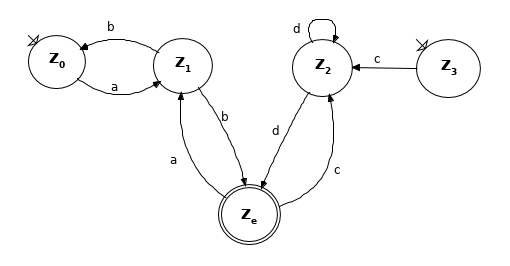
\includegraphics[scale=0.6]{G-6-A-02-Buczko_Heid_Deinert-Automat1.png}
\subsection{}
\subsubsection{}
Verfahren:
\begin{enumerate}
\item Die beiden Automaten werden nebeneinander aufgemalt
\item Jede Kante, die einen Zyklus im Ursprungsautomaten beendet, wird kopiert 
und zu allen weiteren Startzuständen umgebogen
\end{enumerate}
\subsubsection{}
Termination:\\
Da beide Automaten endliche viele Kanten, die Zyklen beenden können haben, 
müssen nur endlich viele Kanten kopiert und zu endlich vielen Zuständen 
umgebogen werden. Dieses terminiert somit in endlicher Zeit.
\\\\
Korrektheit:\\
Da der Zweite teil eines Wortes im neuen Automaten gleich dem vollständigen akzpetierten Wort des Ursprungsautomaten ist, ergibt sich die Korrektheit daraus, dass vom ersten Teil des Wortes in den zweiten Ursprungsautomat gewechselt und somit das urspünglich akzpetierte Wort gelesen werden kann.  
\end{document}
